\RequirePackage[l2tabu, orthodox]{nag}
%\pdfminorversion=4
\documentclass[a0paper,portrait,fontscale=0.35]{baposter}

\usepackage{amsfonts,amsmath,amsthm,amssymb,commath}
\usepackage{graphicx,subcaption}
\usepackage[most,skins,theorems]{tcolorbox}
\usepackage{color}
\usepackage[none]{hyphenat} 

\usepackage{relsize}
\usepackage{natbib}
\usepackage{microtype}

\usepackage{tikz}
\usetikzlibrary{decorations.pathreplacing}

\usepackage{natbib}
\setlength{\bibsep}{0.0pt}

\newcommand{\PSF}{\text{PSF}}
\newcommand{\argmin}{\text{argmin}}

%%% Define a caption font
\newcommand{\mycaption}[1]{
  {
    \smaller
    \emph{#1}
  }
}

\theoremstyle{plain}
\newtheorem{thm}{\protect\theoremname}
  \theoremstyle{plain}
  \newtheorem{lem}[thm]{\protect\lemmaname}
  \theoremstyle{definition}
  \newtheorem{defn}[thm]{\protect\definitionname}
  \theoremstyle{plain}
  \newtheorem{prop}[thm]{\protect\propositionname}
  \theoremstyle{definition}
  \newtheorem{example}[thm]{\protect\examplename}

%%% Color Definitions %%%%%%%%%%%%%%%%%%%%%%%%%%%%%%%%%%%%%%%%%%%%%%%%%%%%%%%%%
%\definecolor{oxford_blue}{RGB}{14,31,71}
%\definecolor{oxford_border}{RGB}{14,31,71}

%\definecolor{cambridge_blue}{RGB}{64,76,0}
%\definecolor{cambridge_blue}{RGB}{163, 193, 173}
%\definecolor{cambridge_border}{RGB}{163, 193, 173}

\definecolor{cambridge_blue}{RGB}{49,72,56}
\definecolor{cambridge_border}{RGB}{49,72,56}

\tcbset{highlight math style={enhanced, 
    colframe=cambridge_blue, colback=white}}

\begin{document}
\typeout{Poster rendering started}

\begin{poster}
{
    % Show grid to help with alignment
    grid=false,
    columns=6,
    % Column spacing
    colspacing=0.7em,
    % Color style
    %headerColorOne=cyan!20!white!90!black,
    %borderColor=cyan!30!white!90!black,
    headerColorOne=cambridge_blue,
    borderColor=cambridge_border,
    headerFontColor=white,
    % Format of textbox
    textborder=faded,
    % Format of text header
    headerborder=open,
    headershape=smallrounded,
    headershade=plain,
    background=none,
    bgColorOne=cyan!10!white,
    %headerheight=0.11\textheight,
    headerheight=0.095\textheight,
    eyecatcher=false,
}
% Eye Catcher: Oxford logo and personal picture
{
%  \makebox[0.23\textwidth]{
%    \begin{tabular}{cc}
%    
\includegraphics[height=0.055\textheight]{./img/InFoMM}
%      &
%    %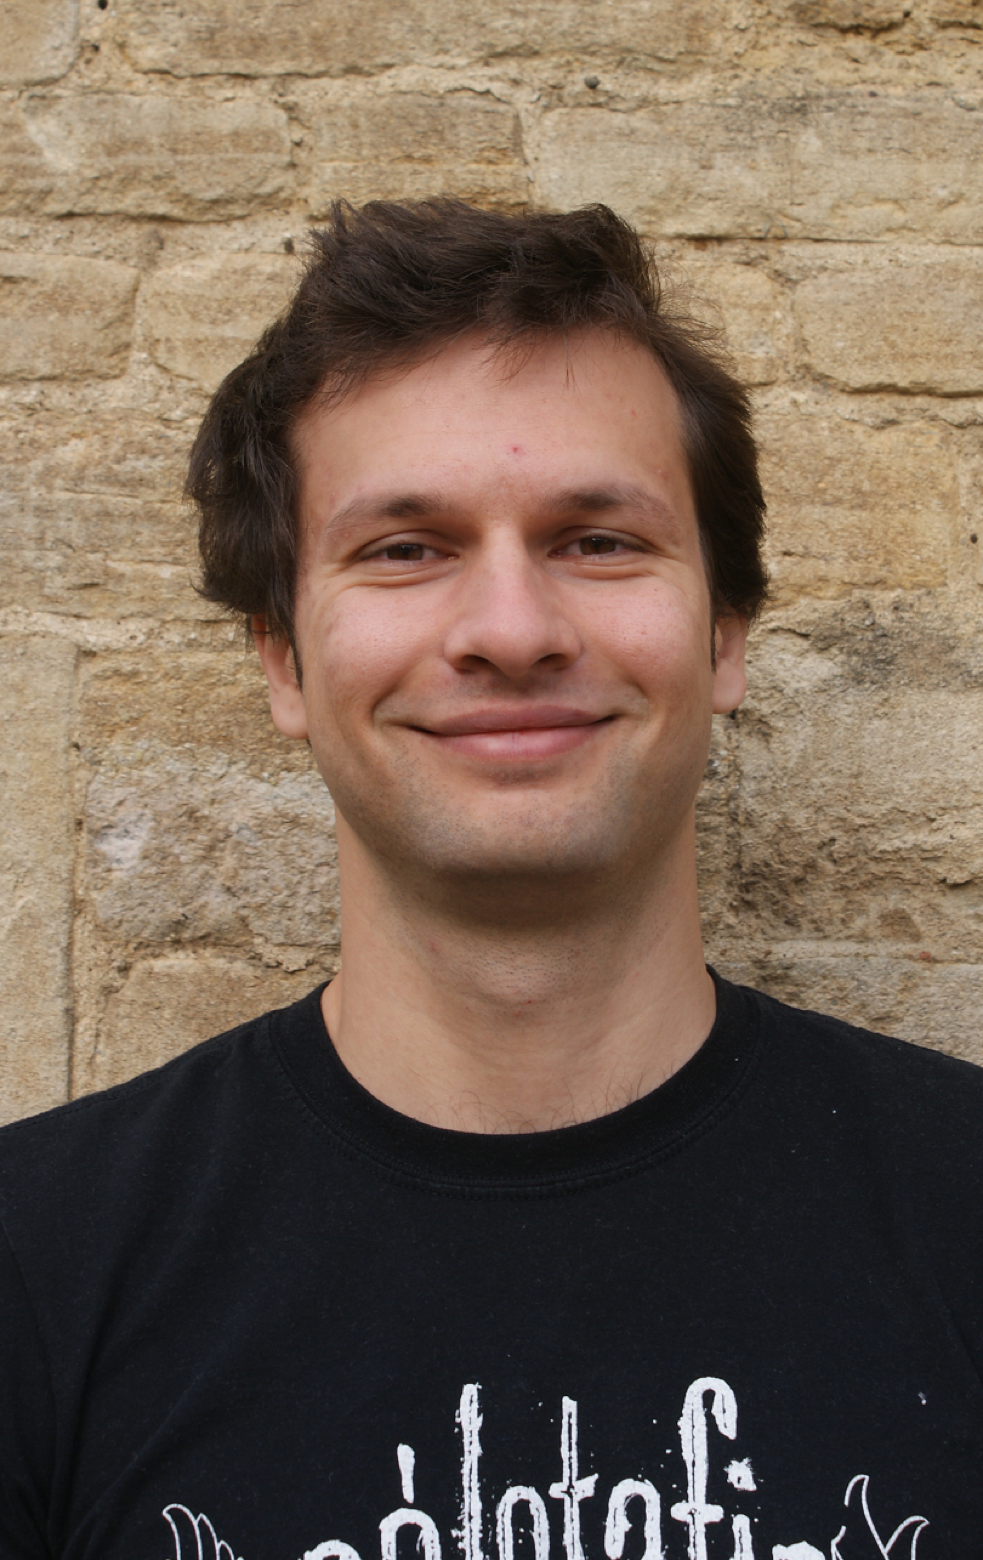
\includegraphics[height=0.10\textheight]{./img/me}
%    \end{tabular}
%    \hfill
%  }
}
%%% Title %%%%%%%%%%%%%%%%%%%%%%%%%%%%%%%%%%%%%%%%%%%%%%%%%%%%%%%%%%%%%%%%%%%%%
{
  %%\textsc{Source Reconstruction \vspace{0.2cm}\\From Hydrophone Data}
  \textsc{Spatially Variable Deconvolution\vspace{0.2cm}\\ 
    for Light-sheet Microscopy\vspace{0.2em}}
  %\vspace{0.3em}
}
%%% Authors %%%%%%%%%%%%%%%%%%%%%%%%%%%%%%%%%%%%%%%%%%%%%%%%%%%%%%%%%%%%%%%%%%%
{
  \vspace{0.1em}
  \hspace{-0.65em}
  {
    \underline{\textbf{Bogdan Toader}}\textsuperscript{1},
    \textbf{J\'{e}r\^{o}me Boulanger}\textsuperscript{2},
    \textbf{Yury Korolev}\textsuperscript{1},
    \textbf{Martin Lenz}\textsuperscript{1},\\
    \textbf{James Manton}\textsuperscript{2},
    \textbf{Leila Mure\c{s}an}\textsuperscript{1},
    \textbf{Carola-Bibiane Sch\"{o}nlieb}\textsuperscript{1}
  } \\[0.2em]
  {
    \textsuperscript{1}University of Cambridge,
    \textsuperscript{2}MRC Laboratory of Molecular Biology 
  }
  \vspace{-1em}
}
%%% InFoMM Logo %%%%%%%%%%%%%%%%%%%%%%%%%%%%%%%%%%%%%%%%%%%%%%%%%%%%%%%%%%%%%%%
%{
%  %\makebox[0.23\textwidth]{
%  \makebox[0.32\textwidth]{
%    \hfill
%    \begin{tabular}{ccc}
%    %
\includegraphics[height=0.055\textheight]{./img/InFoMM}
%      
\includegraphics[height=0.04\textheight]{./img/InFoMM}
%      &
%    %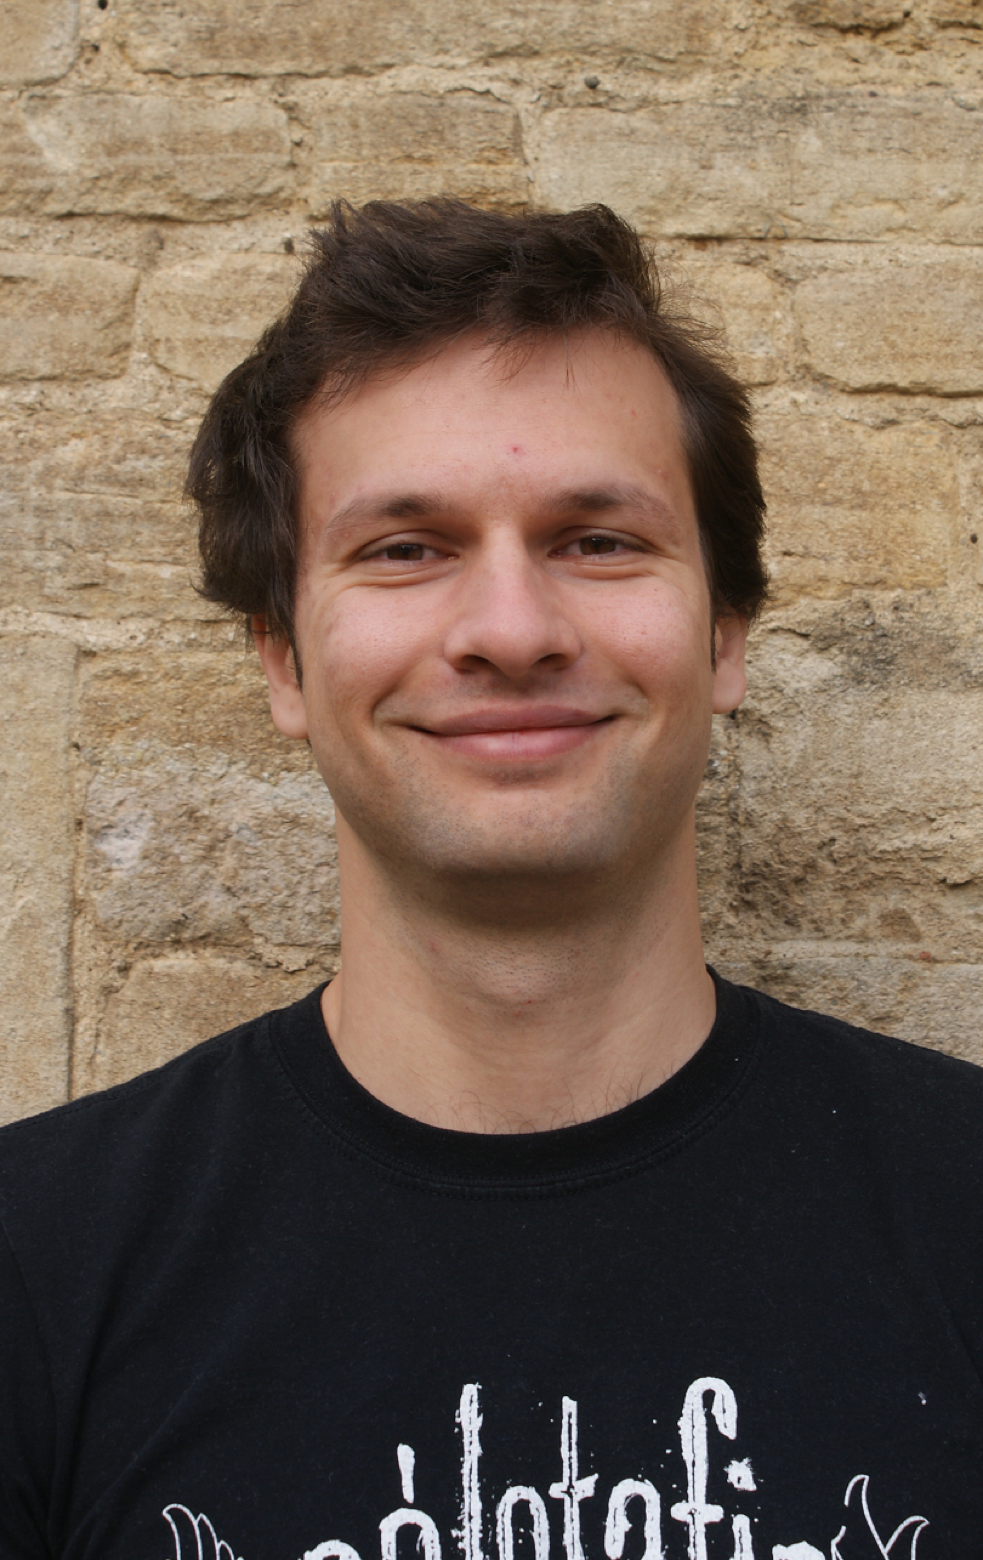
\includegraphics[height=0.10\textheight]{./img/me}
%      
\includegraphics[height=0.04\textheight]{./img/oxlogo}
%      \\
%      
\includegraphics[height=0.04\textheight]{./img/turinglogo2}
%      &
%      
\includegraphics[height=0.04\textheight]{./img/edinlogo}
%      %&
%      %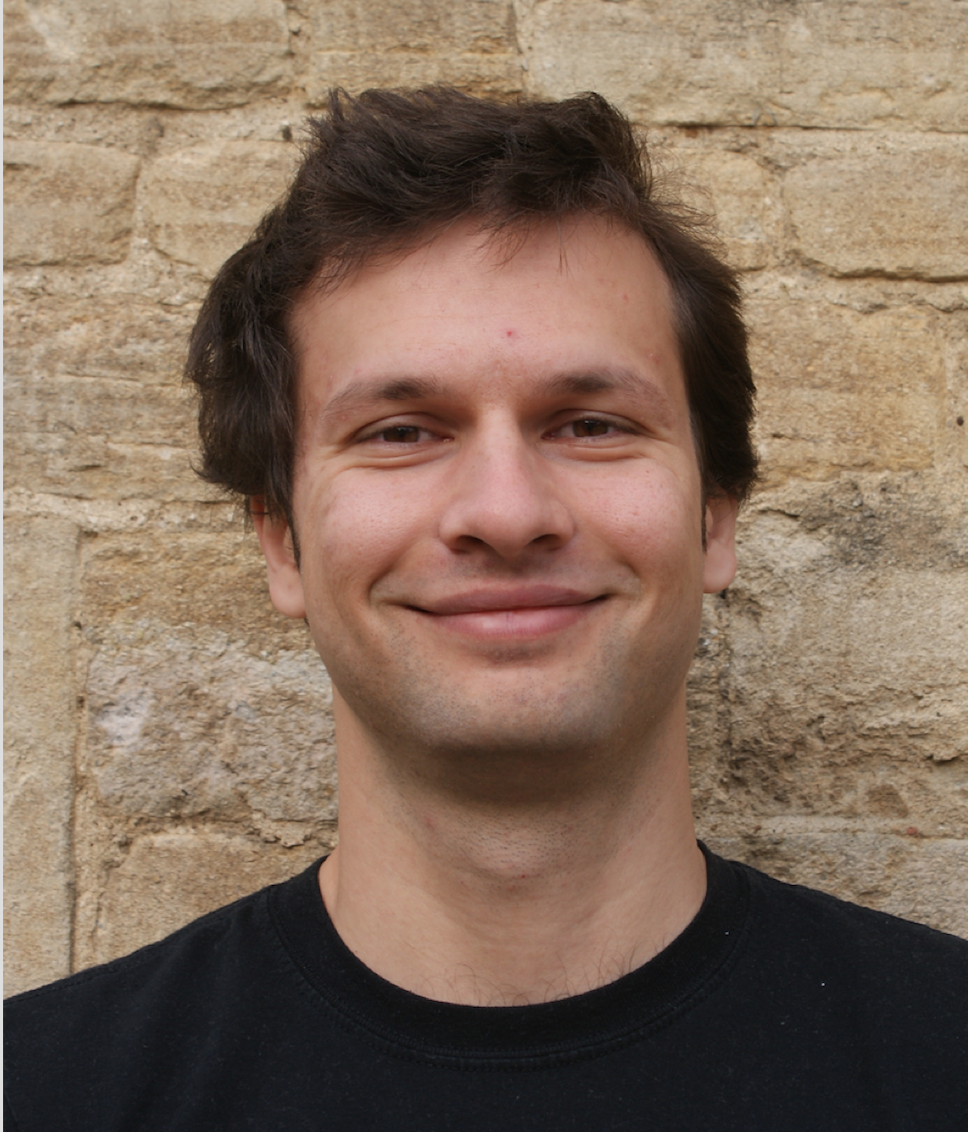
\includegraphics[height=0.05\textheight]{./img/me_square}
%    \end{tabular}
%  }
%  %}
%}
{
  %\makebox[0.23\textwidth]{
  \makebox[0.32\textwidth]{
    \hfill
    \begin{tabular}{ccc}
      
\includegraphics[height=0.04\textheight]{./img/camlogo}
    \end{tabular}
  }
  %}
}
\headerbox{lightsheet microscopy}{name=lightsheet, span=3, column=0, row=0}{
  Light-sheet microscopy is a type of fluorescence 
  microscopy used in cell biology due to its fast 
  acquisition times and low photo-damage to the sample. 
  This is achieved by selectively illuminating a slice 
  of the sample using a sheet of light and detecting the 
  emitted fluorescence signal using a dedicated 
  objective orthogonal to the plane of the sheet. 
  \vspace{1pt}
  \begin{minipage}[t]{0.48\textwidth}
    \centering
    \raisebox{\dimexpr-\height+\ht\strutbox}{
      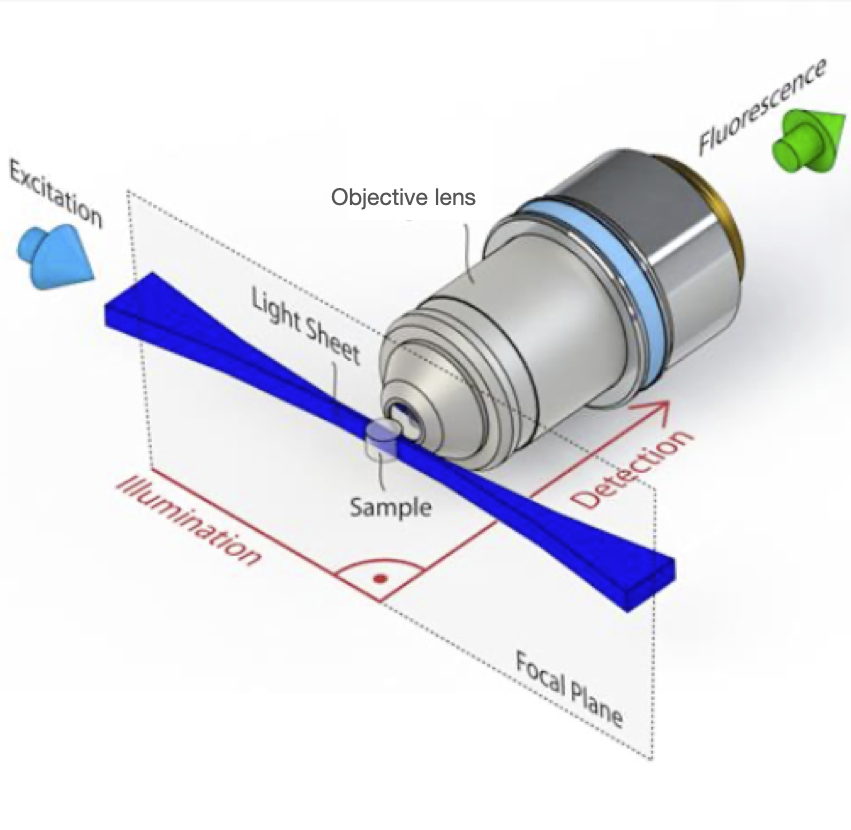
\includegraphics[width=0.8\textwidth]{img/spim.png}
    }
   
    \mycaption{Figure credit: J\"{o}rg Ritter, PhD thesis (2011)}
  \end{minipage}
  %
  \begin{minipage}[t]{0.48\textwidth}
    \begin{center}
      \larger
      {\color{blue}\textbf{\textsc{spatially varying psf}}}\\
      %\textit{$y_i$ are the samples\\
      %  we use to reconstruct $x$.}
    \end{center}
    
    \begin{minipage}[t]{\textwidth}
      \centering
      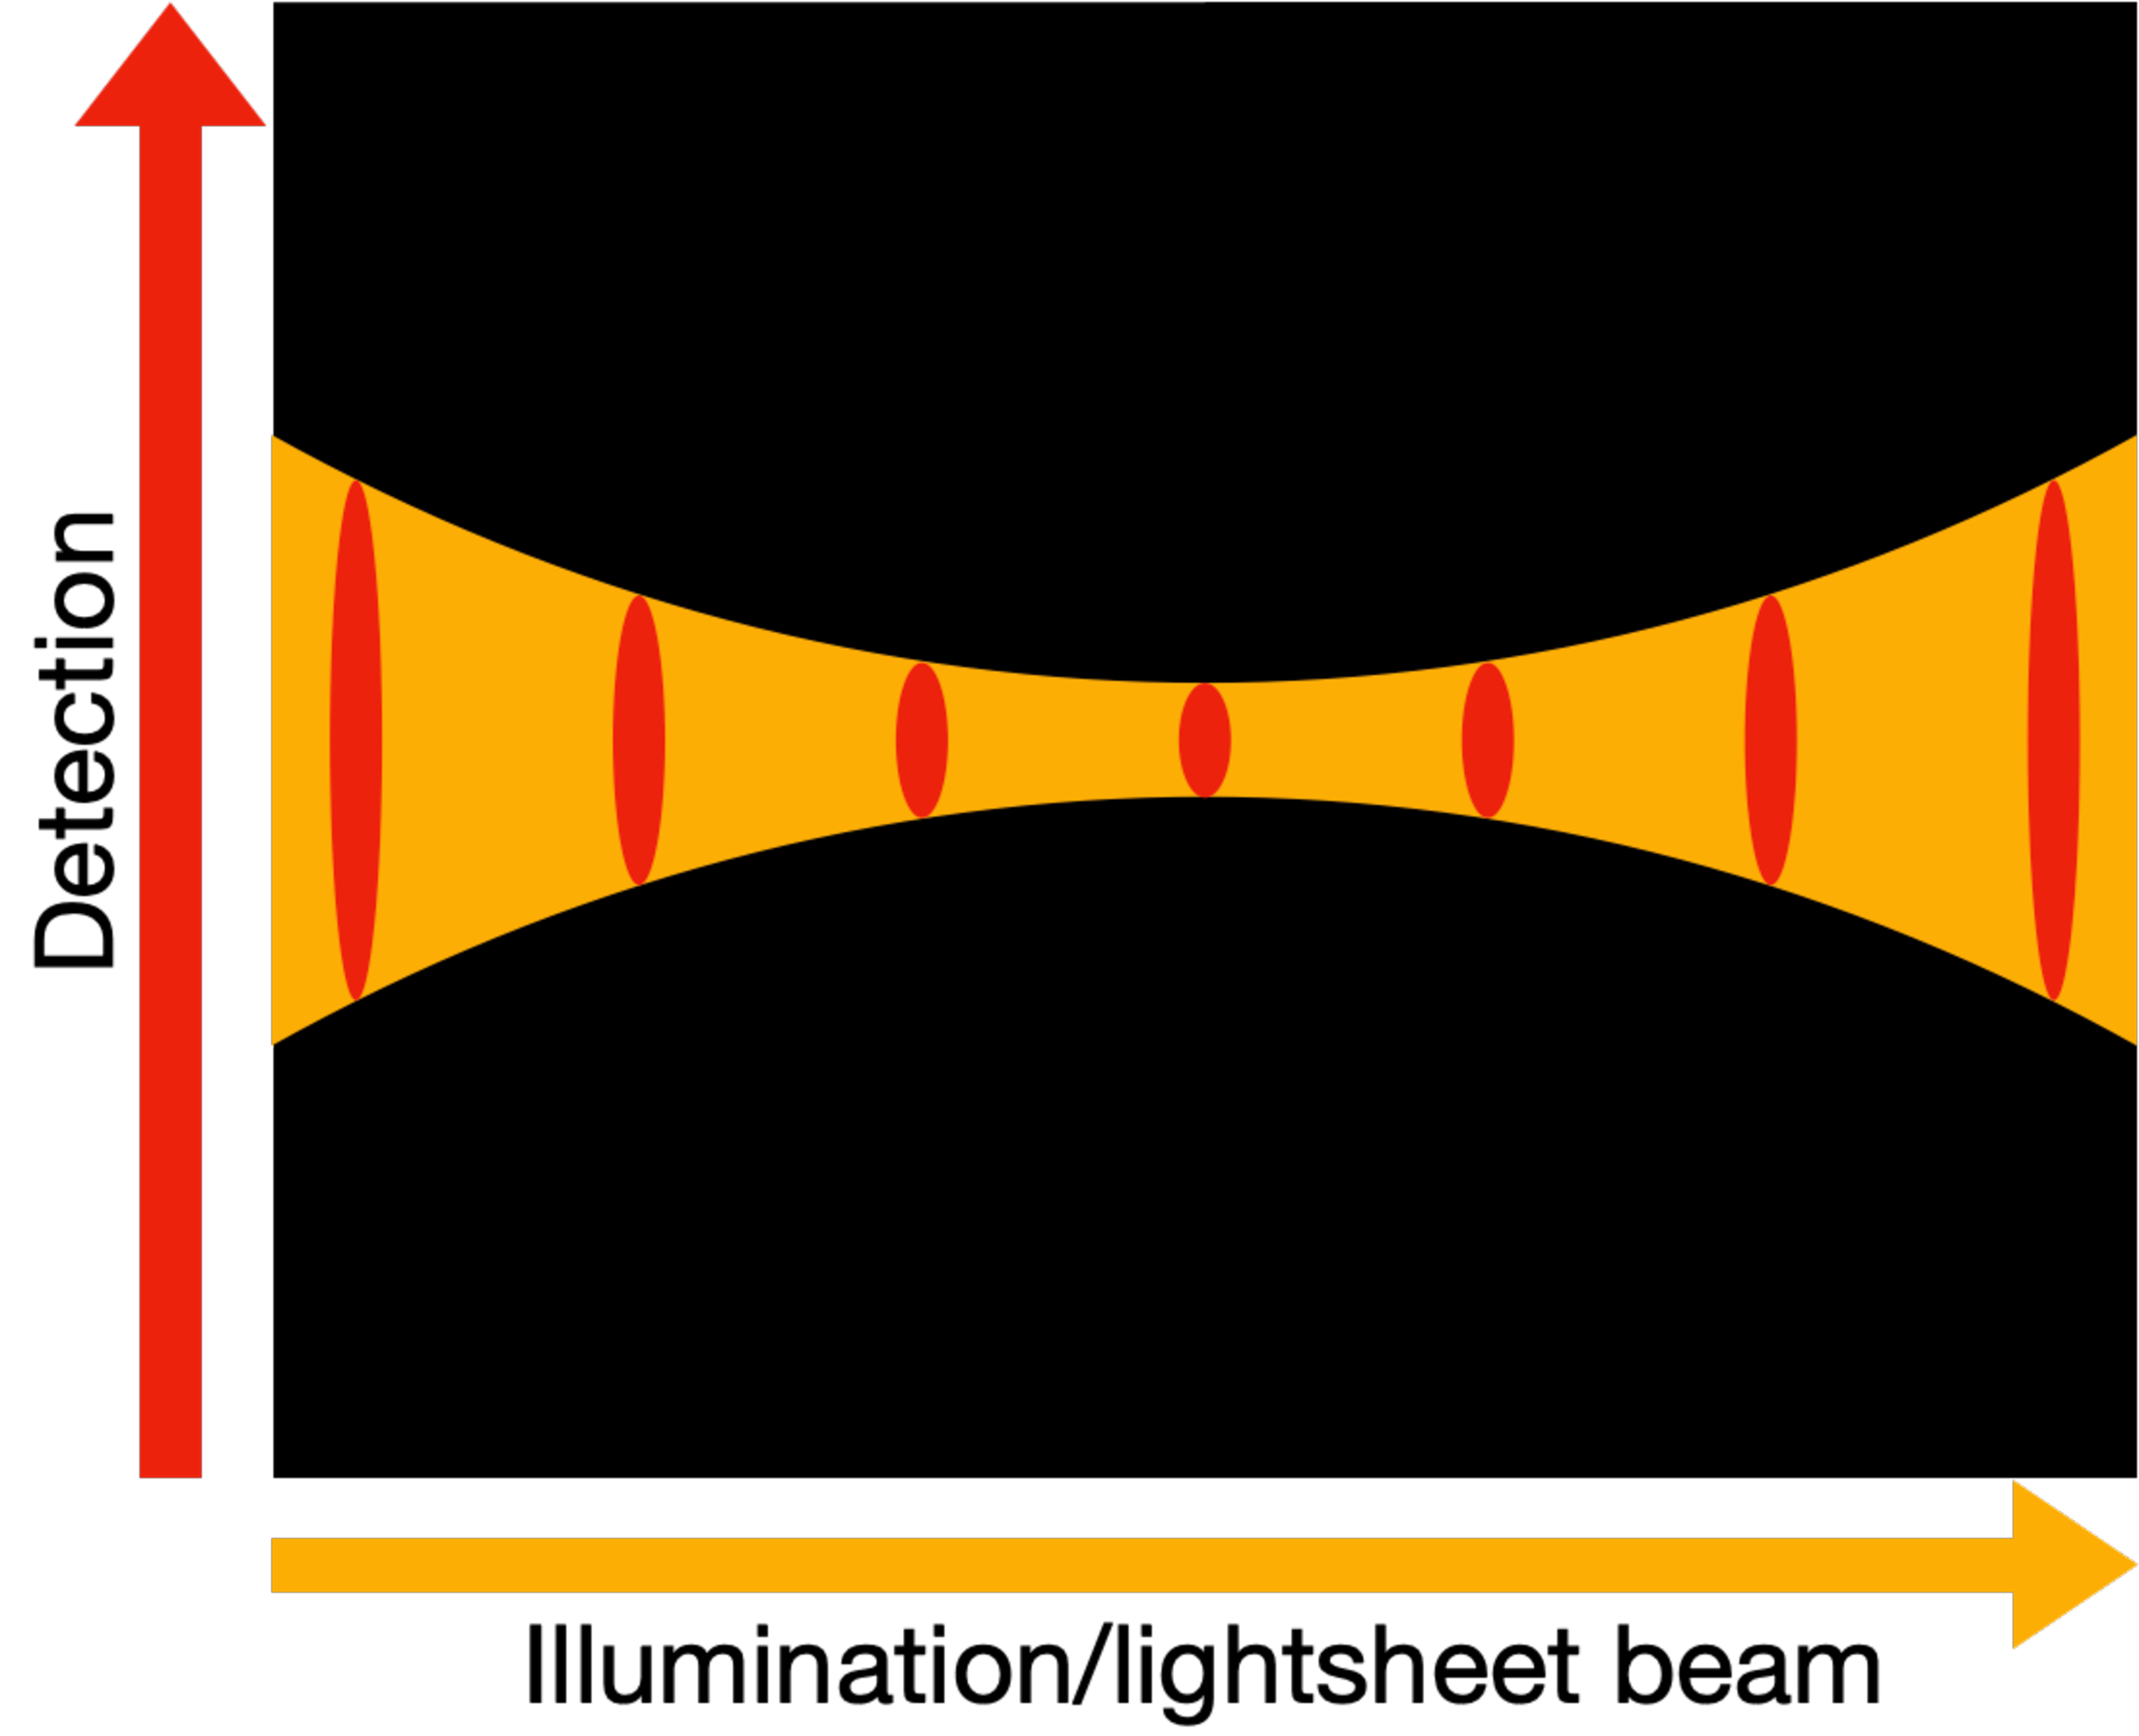
\includegraphics[width=\textwidth]{img/psf_vary.pdf}
    \end{minipage}
  \end{minipage}
     
  \begin{minipage}[t]{0.48\textwidth}
    \begin{center}
      \larger
      {\color{red}\textbf{\textsc{problem}}}\\
    \end{center}
    \vspace{-1em}
    \begin{tcolorbox}[colback=red!10!white,colframe=red]
      Due to the interaction of the light-sheet beam  
      and the detection/objective point spread function (PSF), 
      the effective PSF of the system is spatially varying, and
      therefore standard deconvolution approaches are not applicable.
    \end{tcolorbox}
  \end{minipage}
  %
  \hspace{0.6em}
  \begin{minipage}[t]{0.48\textwidth}
    %\vspace{-1em}
    \begin{center}
      \larger
      {\color{blue}\textbf{\textsc{goal}}}\\
    \end{center}
    \vspace{-1em}
    \begin{tcolorbox}[colback=blue!10!white,colframe=blue]
      In this work, we propose a model for image formation 
      that describes the interaction between the 
      illumination PSF and the detection PSF which 
      replicates the physics of the microscope while 
      leading to a tractable inverse problem.
    \end{tcolorbox}
  \end{minipage}
  \vspace{-1em}
}
\headerbox{psf model}{name=psf, span=3, column=3, row=0}{

  \begin{minipage}[t]{\textwidth}
    The detection PSF $h$ is modelled as the Fourier
    transform of the pupil function multiplied by 
    defocus~\cite{Stokseth1969}: 
    \begin{tcolorbox}[colback=teal!10!white,colframe=white]
      \vspace{-1em}
      \begin{equation}
        h(x,y,z) = \left|
          \iint g_{\sigma} * p(\kappa_x,\kappa_y) e^{
            2 i \pi z 
            \sqrt{(n/\lambda)^2 - \kappa_x^2 - \kappa_y^2}
          }
          e^{
            2 i \pi (\kappa_x x + \kappa_y y)
          }
          \dif \kappa_x \dif \kappa_y
        \right|^2
        \label{eq:psf model}
      \end{equation}
    \end{tcolorbox}
    where $p$ is the pupil function, defined as
    \begin{tcolorbox}[colback=teal!10!white,colframe=white]
      \begin{equation}
        p(\kappa_x,\kappa_y) = \begin{cases}
          e^{2i\pi \sum_{j=1}^{15} c_i Z_j(\kappa_x,\kappa_y)}
          \quad
            &\text{for} \quad
            \rho = \sqrt{\kappa_x^2 + \kappa_y^2} \leq NA/\lambda,\\
            0, \quad &\text{otherwise.}
        \end{cases}
      \end{equation}
    \end{tcolorbox}
    where the phase of the pupil function is computed by least-squares
    fitting of the coefficients of the first $15$ Zernike polynomials
    using an image of a bead.
  \end{minipage}

  \vspace{10pt}
  \begin{minipage}[t]{\textwidth}
    \begin{minipage}[t]{0.38\textwidth}
      The parameters of the model are given by
      the experimental setup used to acquire the image:
      \begin{itemize}
        \item $n$ - refractive index
        \item $\lambda$ - wave length
        \item NA - numerical aperture
        \item $g_{\sigma}$ Gaussian blur to take into account
          other properties not accounted for in our model
      \end{itemize}
    \end{minipage}
    %
    \begin{minipage}[t]{0.3\textwidth}
      \centering
      \raisebox{\dimexpr-\height+\ht\strutbox}{
        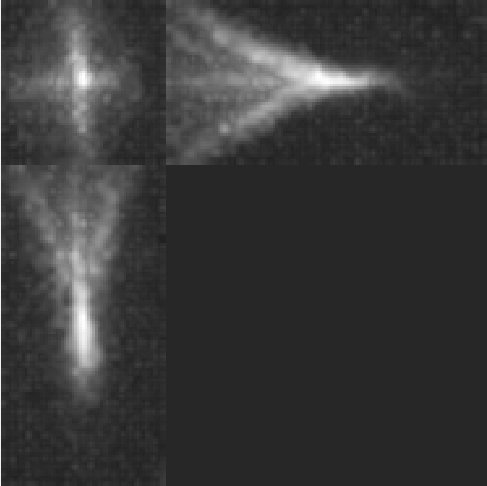
\includegraphics[height=0.1\textheight]{img/psf_bead.png}
      }

      \vspace{0.3em}
      \mycaption{
        Bead image (MIP)
      }
    \end{minipage}
    %
    \begin{minipage}[t]{0.3\textwidth}
      \centering
      \raisebox{\dimexpr-\height+\ht\strutbox}{
        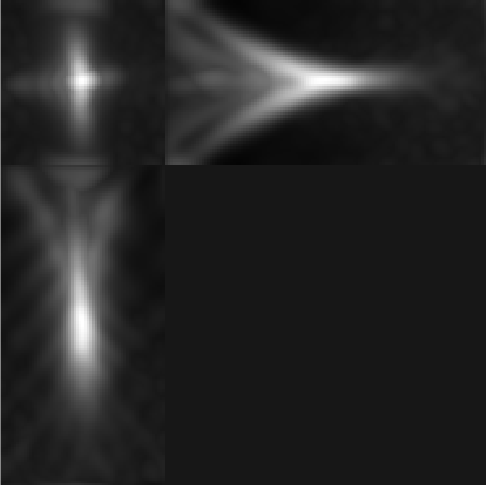
\includegraphics[height=0.1\textheight]{img/psf_zernike_sigma.png}
      }

      \vspace{0.3em}
      \mycaption{
        Estimated detection PSF (MIP)
      }
    \end{minipage}
  \end{minipage} 
}

\headerbox{image formation model}{name=model, span=3, column=0, below=lightsheet}{
  %\begin{minipage}[t]{\textwidth} 

    The sample $s$ illuminated at $z=z_0$ by the light-sheet $l$
    and the photons are collected by an objective with PSF $h$:
    \vspace{0.5em} 
    
    \begin{minipage}[t]{\textwidth}
      \centering
      \raisebox{\dimexpr-\height+\ht\strutbox}{
        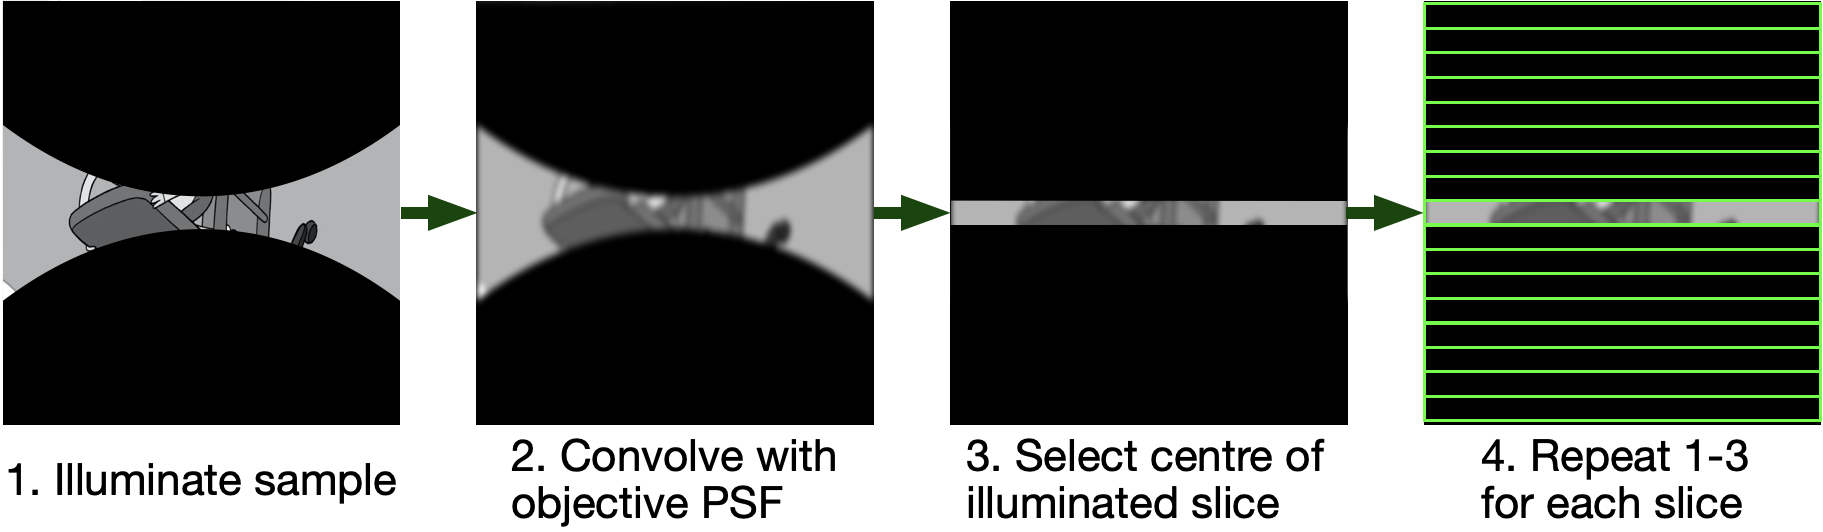
\includegraphics[height=0.094\textheight]{img/model_diags.png}
      }
    \end{minipage}

    \begin{tcolorbox}[colback=teal!10!white,colframe=white]
      \vspace{-1em}
      \begin{equation}
        f(x,y,z_0) = \iiint l_{avg_y}(u,v,w) s(u,v,w - z_0) h(x-u,y-v,w) \dif u \dif v \dif w
        \label{eq:lightsheet model}
      \end{equation}
    \end{tcolorbox}
    where $h$ is the detection PSF, calculated using \eqref{eq:psf model} 
    and $l_{avg_y}$ is the light-sheet, calculated by averaging the beam
    PSF obtained in a similar way to $h$, without Zernike polynomials.

    \vspace{0.5em}
    \begin{minipage}[t]{\textwidth}
      \centering
      \raisebox{\dimexpr-\height+\ht\strutbox}{
        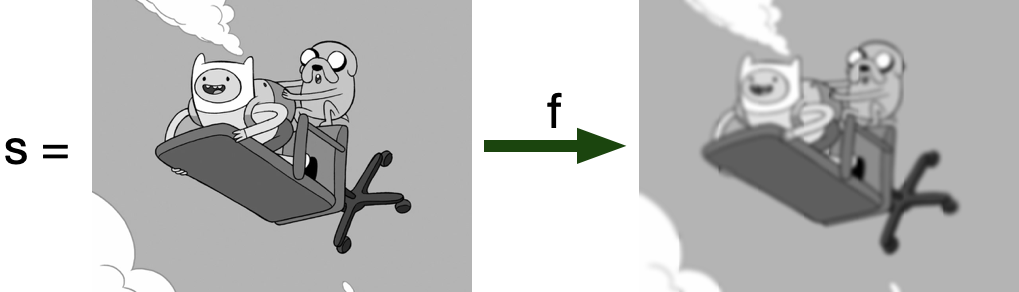
\includegraphics[height=0.065\textheight]{img/f_to_s.png}
      }
    \end{minipage}
    
    \vspace{-0.5em}

 % \end{minipage}
}

\headerbox{reconstruction}{name=resultssim, span=3, column=3, below=lightsheet}{
    Let $\hat{f}$ be the image data with Gaussian noise
    and $f(s)$ the result of applying the forward
    model \eqref{eq:lightsheet model} to the sample $s$.
    To recover $s$, we solve:
    \vspace{-0.5em}
    \begin{tcolorbox}[colback=red!10!white,colframe=white]
      \begin{equation}
        \text{Find }
        \hat{s} \in 
        \argmin_{s} \left\{
          \| \hat{f} - f(s)   \|_{L_2}
          + \lambda TV(s)  
        \right\}
        \label{eq:min prob}
      \end{equation}
    \end{tcolorbox}
    \vspace{-0.5em}

    \begin{minipage}[t]{0.55\textwidth}
      \begin{minipage}[t]{0.49\textwidth}
        \centering

        \raisebox{\dimexpr-\height+\ht\strutbox}{
          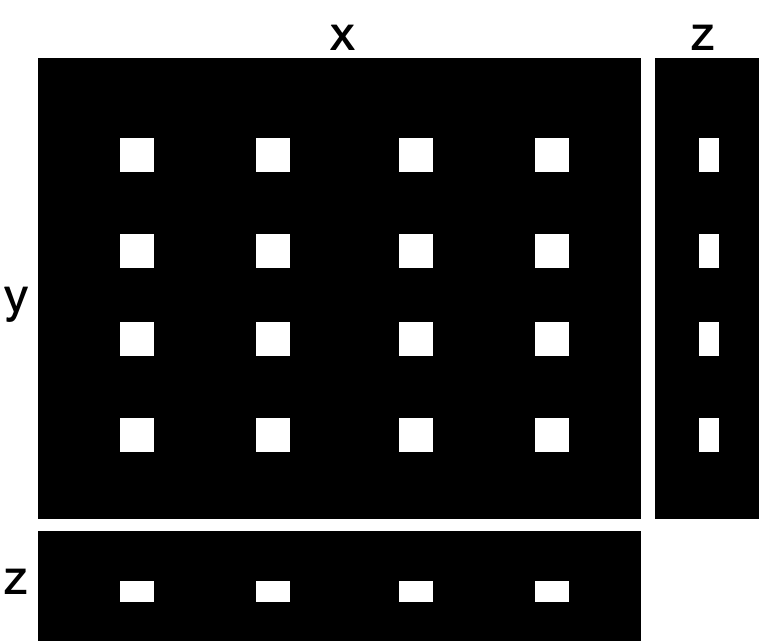
\includegraphics[height=0.08\textheight]{img/simulated/u0_mod}
        }
        \vspace{0.3em}
        \mycaption{
          (a) Ground truth image
        }
      \end{minipage}
      %
      \begin{minipage}[t]{0.49\textwidth}
        \centering

        \raisebox{\dimexpr-\height+\ht\strutbox}{
          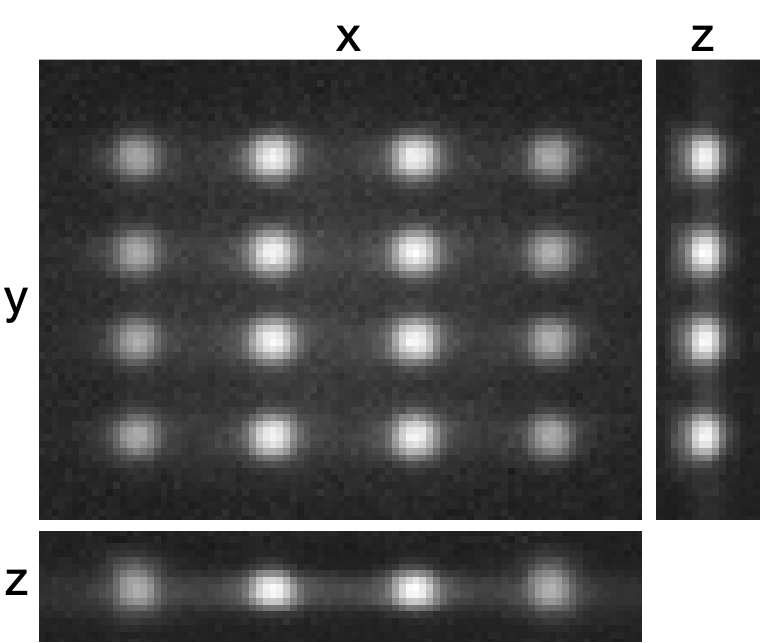
\includegraphics[height=0.08\textheight]{img/simulated/f_gaussian_mod}
        }
        \vspace{0.3em}
        \mycaption{
          (b) Data 
        }
      \end{minipage}

      %\vspace{0.9em}
      \begin{minipage}[t]{0.49\textwidth}
        \centering

        \raisebox{\dimexpr-\height+\ht\strutbox}{
          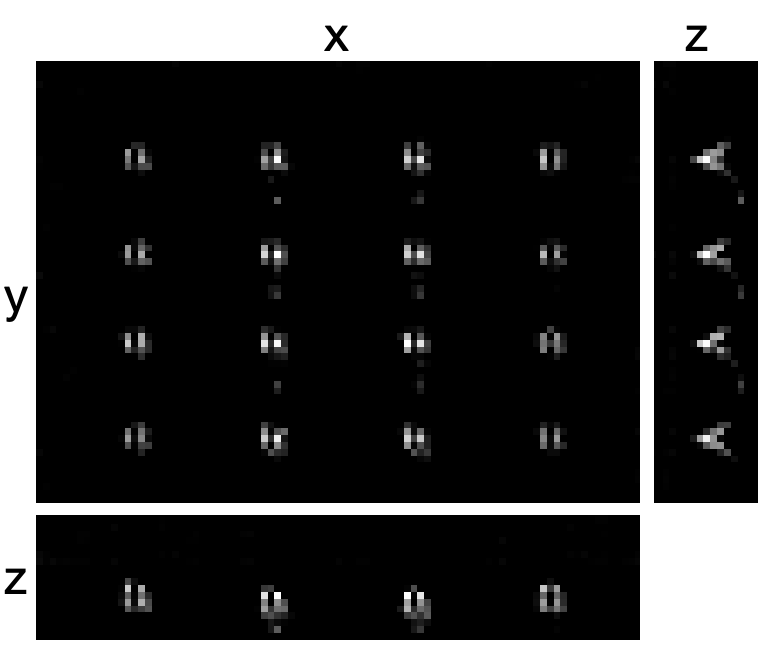
\includegraphics[height=0.08\textheight]{img/simulated/gauss_urec_h_mod}
        }
        \vspace{-0.3em}
        \mycaption{
          (c) Constant PSF deconvolution 
        }
      \end{minipage}
      %
      \begin{minipage}[t]{0.49\textwidth}
        \centering

        \raisebox{\dimexpr-\height+\ht\strutbox}{
          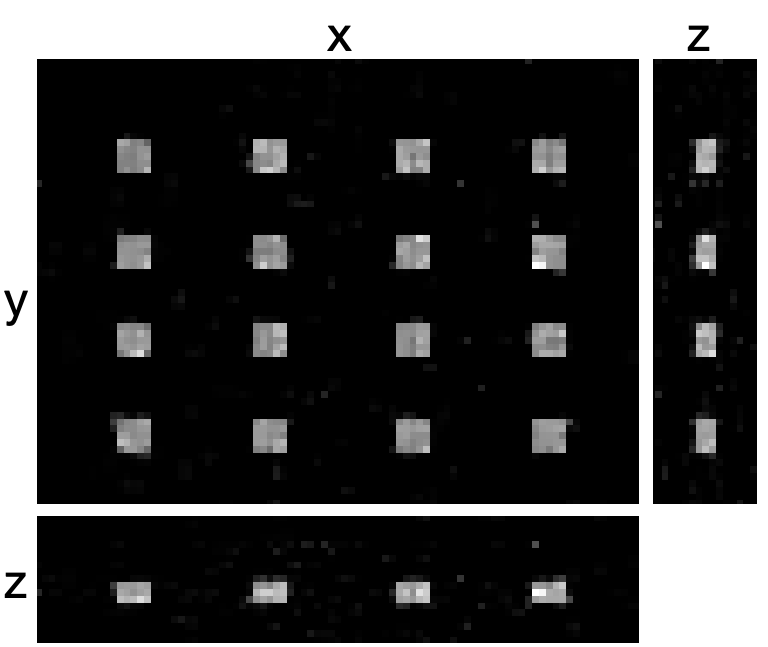
\includegraphics[height=0.08\textheight]{img/simulated/gauss_urec_l_mod}
        }

        \vspace{0.3em}
        \mycaption{
          (d) Model deconvolution
        }
      \end{minipage}
    \end{minipage}
    %
    \hspace{-0.5em}
    \begin{minipage}[t]{0.45\textwidth}
      \begin{itemize}
        \item We use the total variation regulariser $TV(s)$
          and $\ell_2$ fidelity term due to the Gaussian
          noise in the data. 

        \item To solve the optimisation problem, we apply a version
          of the Primal Dual Hybrid Gradient (PDHG) 
          algorithm from \cite{Boulanger2018,Condat2013}.

        \item In the figure on the left, we show an example of a simulated sample (a) 
          to which we apply the forward model with Gaussian noise (b)
          and the result of deconvolving using only a spatially varying
          PSF (c) and the full forward model (d). 

        \item The images are shown 
          using maximum intensity projection.
      \end{itemize}
    \end{minipage}
}

\headerbox{results}
{name=resultsreal,column=0, below=model, span=6}{
  \begin{minipage}[t]{0.33\textwidth} 
 
    \vspace{1em}
    We solve the minimisation problem \eqref{eq:min prob}
    with the forward model given by \eqref{eq:lightsheet model}
    and the PSF model in \eqref{eq:psf model}
    to two 3D image stacks: 
    \begin{enumerate} 
      \item Beads in agarose (1127 x 111 x 100 pixels).

      \item Marchantia plant (1127 x 155 x 100 pixels).
    \end{enumerate}

    We compare our proposed method with deconvolution using
    constant PSF, namely the detection PSF $h$
    estimated in \eqref{eq:psf model}. In this case,
    we solve the same minimisation problem \eqref{eq:min prob}, 
    except that the forward model is only a convolution
    operator.

    \begin{itemize}
      \item In the bead images, the lobes of the beads 
        due to spherical aberration are minimised, as seen
        in the XY slice, while in the XZ slice we see that
        the beads become symmetric and less elongated.

      \item In the Marchantia image, the contrast is 
        enhanced, the cell walls becoming sharper 
        using our proposed approach compared to the constant
        PSF deconvolution.
    \end{itemize}

  \end{minipage}
  %
  \begin{minipage}[t]{0.33\textwidth} 
    \begin{center}
      \larger
      \textbf{\textsc{1. beads}}
    \end{center}

    \vspace{-0.5em}
    \centering
    \begin{minipage}[t]{0.85\textwidth}
      \centering
      \raisebox{\dimexpr-\height+\ht\strutbox}{
        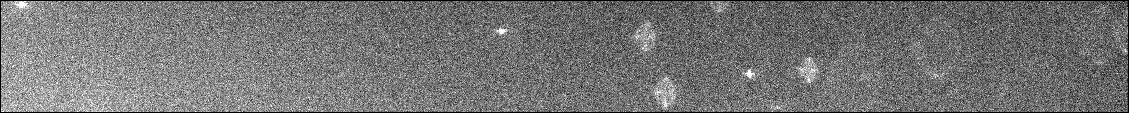
\includegraphics[width=\textwidth]{img/fBeads_xy1.png}
      }
      \raisebox{\dimexpr-\height+\ht\strutbox}{
        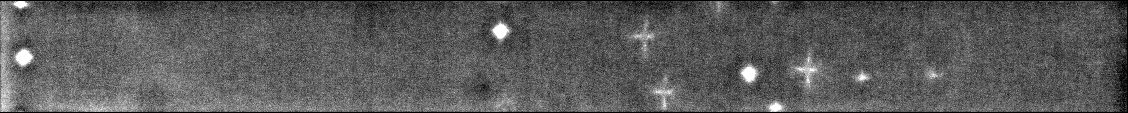
\includegraphics[width=\textwidth]{img/urecBeads_h_xy1.png}
      }
      \raisebox{\dimexpr-\height+\ht\strutbox}{
        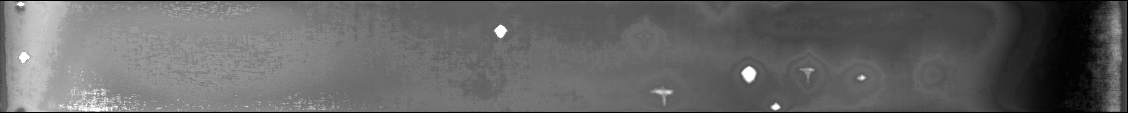
\includegraphics[width=\textwidth]{img/urecBeads_xy1.png}
      }

      \vspace{-1em}
      \begin{center}
        \mycaption{
          XY slice: 
          data (top), constant PSF deconvolution (middle),
          model deconvolution (bottom)
        }
      \end{center}

      \vspace{-0.5em}
      \centering
      \raisebox{\dimexpr-\height+\ht\strutbox}{
        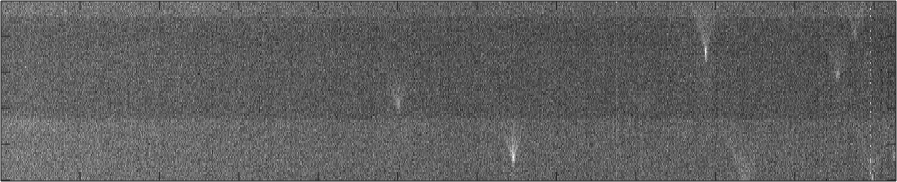
\includegraphics[width=\textwidth]{img/fBeads_xz1.png}
      }
      \raisebox{\dimexpr-\height+\ht\strutbox}{
        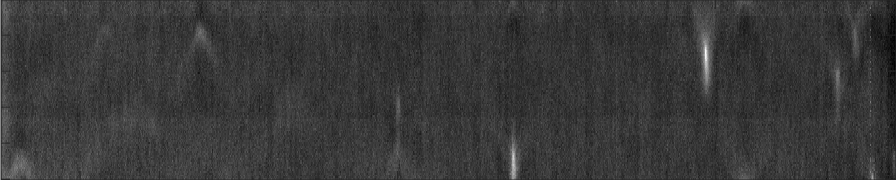
\includegraphics[width=\textwidth]{img/urecBeads_h_xz1.png}
      }
      \raisebox{\dimexpr-\height+\ht\strutbox}{
        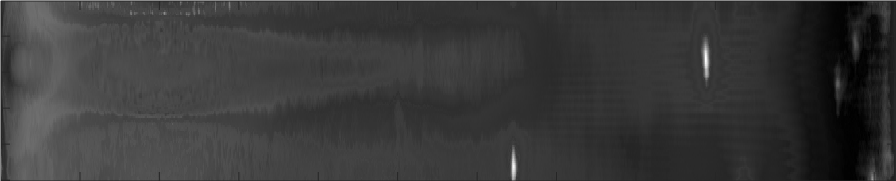
\includegraphics[width=\textwidth]{img/urecBeads_xz1.png}
      }

      \vspace{-1em}
      \begin{center}
        \mycaption{
          XZ slice:
          data (top), constant PSF deconvolution (middle),
          model deconvolution (bottom)
        }
      \end{center}
    \end{minipage}
  \end{minipage}
  %
  \begin{minipage}[t]{0.33\textwidth}
    \begin{center}
      \larger
      \textbf{\textsc{2. marchantia}}
    \end{center}

    %\hspace{0.6cm}
    \vspace{-0.5em}
    \centering
    \begin{minipage}[t]{0.75\textwidth}
      \centering
      \raisebox{\dimexpr-\height+\ht\strutbox}{
        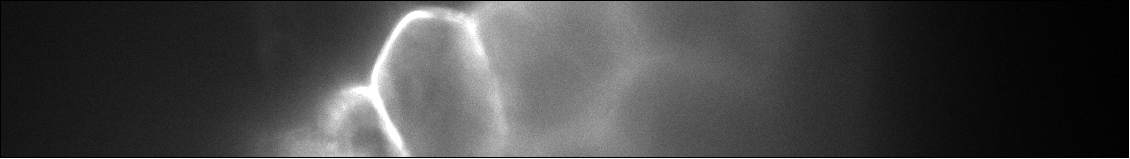
\includegraphics[width=\textwidth]{img/f_xy1.png}
      }
      \raisebox{\dimexpr-\height+\ht\strutbox}{
        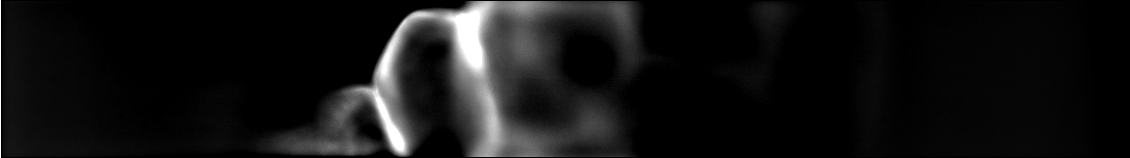
\includegraphics[width=\textwidth]{img/urec_h_xy1.png}
      }
      \raisebox{\dimexpr-\height+\ht\strutbox}{
        
\includegraphics[width=\textwidth]{img/m_urec_it700_lam0p1_xy1.png}
      }

      \vspace{-1em}
      \begin{center}
        \mycaption{
          XY slice: data (top), constant PSF deconvolution (middle),
          model deconvolution (bottom)
        }
      \end{center}

      \vspace{-0.8em}
      \centering
      \raisebox{\dimexpr-\height+\ht\strutbox}{
        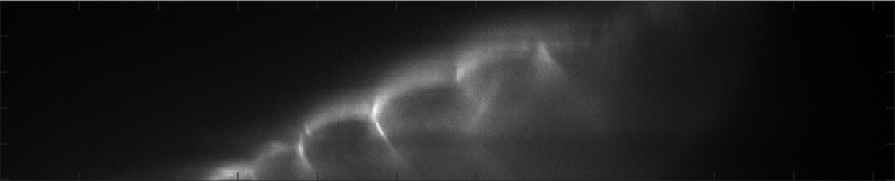
\includegraphics[width=\textwidth]{img/f_xz1.png}
      }
      \raisebox{\dimexpr-\height+\ht\strutbox}{
        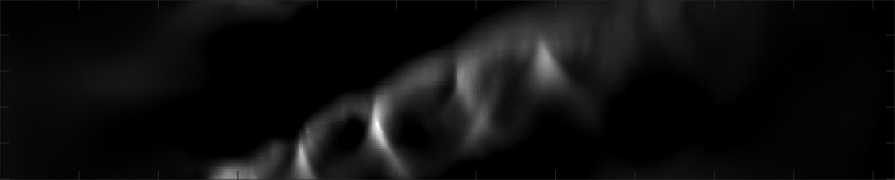
\includegraphics[width=\textwidth]{img/urec_h_xz1.png}
      }
      \raisebox{\dimexpr-\height+\ht\strutbox}{
        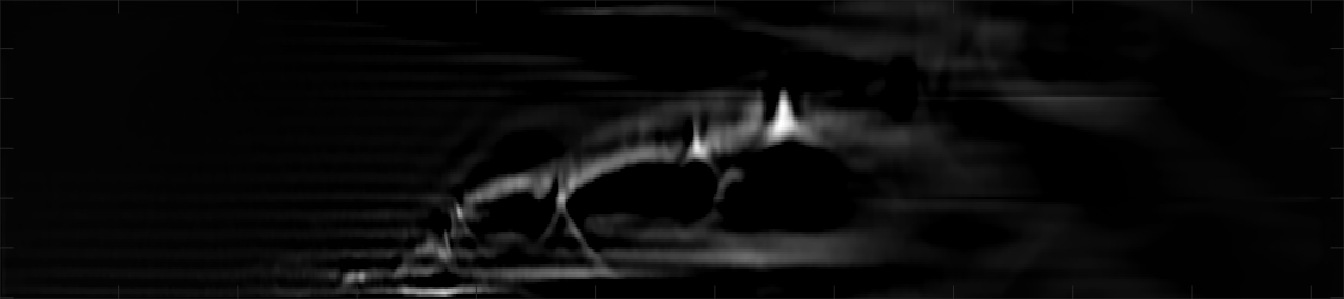
\includegraphics[width=\textwidth]{img/m_urec_it700_lam0p1_xz.png}
      }

      \vspace{-1em}
      \begin{center}
        \mycaption{
          XZ slice: data (top), constant PSF deconvolution (middle),
          model deconvolution (bottom)
        }
      \end{center}
    \end{minipage}
  \end{minipage}
  \vspace{-0.5em}
}

\headerbox{References}
{name=references, column=0,  below=resultsreal, span=4}
%{name=references, column=0,  above=bottom, span=1}
{
  %\smaller                                  % Make the whole text smaller
  %\footnotesize
  %\scriptsize
  \tiny
  \bibliographystyle{abbrv}                 % Use plain style
  \renewcommand{\section}[2]{\vspace{0.01em}}	% Omit "References" title
  \bibliography{references}
}

\headerbox{Acknowledgments}
{name=acknowledgments, column=4, below=resultsreal, span=2}
%{name=acknowledgments, column=1, above=bottom, span=1}
{  
  \scriptsize
  %\tiny
  This work is funded by 
  Isaac Newton Trust/Wellcome Trust ISSF/University of Cambridge 
  Joint Research Grants Scheme, RG89305.

  \par
}






\end{poster}
\end{document}

%%% Local Variables:
%%% mode: latex
%%% TeX-master: t
%%% End:
